\begin{figure*}
\centering
%\subfigure[Disk]{
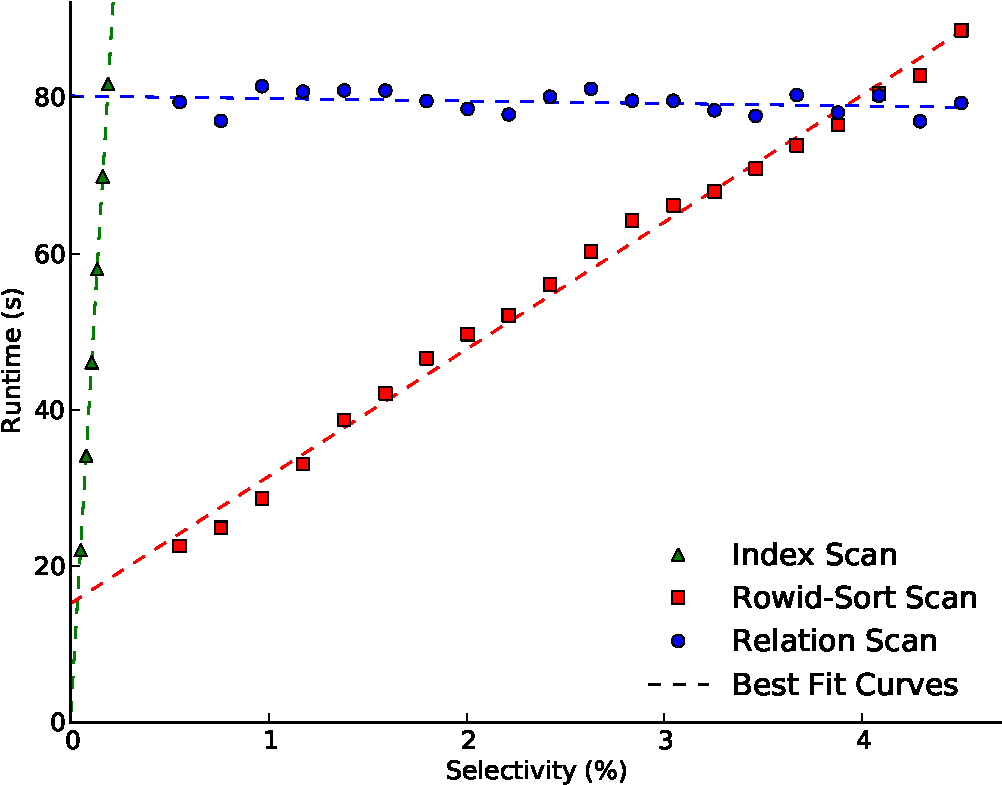
\includegraphics[width=5.0in]{figures/ScanDisk.pdf}
\caption{ \textbf{Scan operator performance on Disk.} Relation scan outperforms the alternatives at selectivities above 4\%, while index scan is optimal only for vanishingly small selectivities (e.g., single-tuple queries).  Best fit curves drawn for convenience.}
\label{fig:scan-disk}
%}
%\hspace{0.5in}
\end{figure*}
\begin{figure*}
\centering
%\subfigure[Flash SSD.]{
  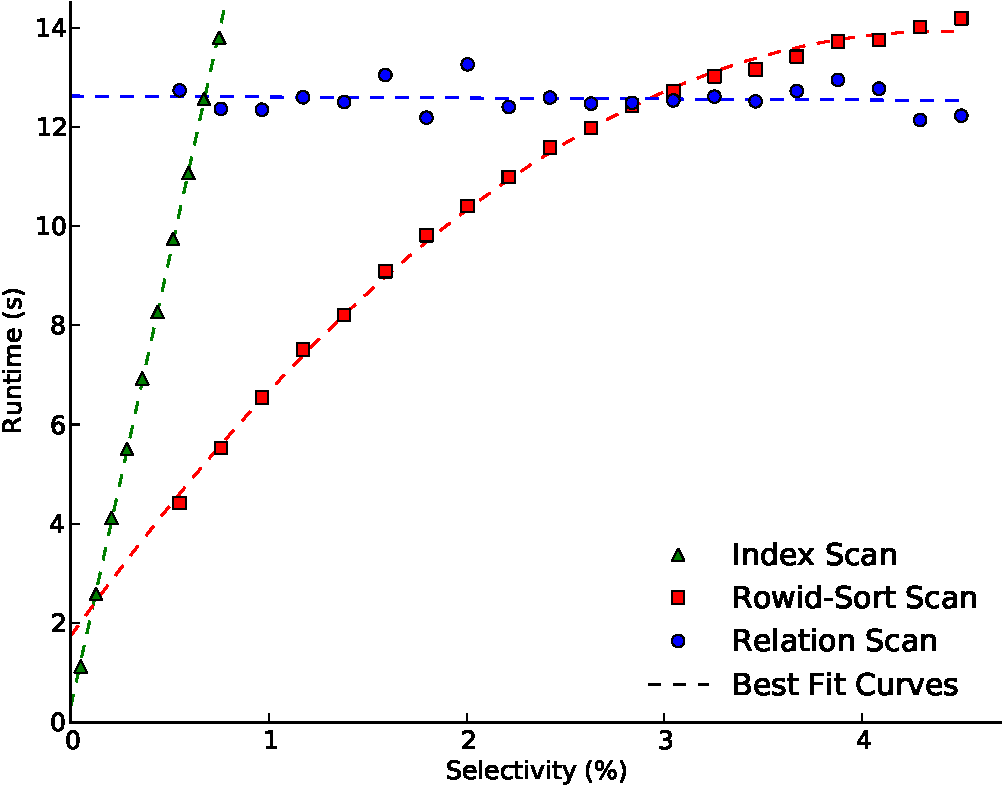
\includegraphics[width=5.0in]{figures/ScanFlash.pdf}
%}
\caption{ \textbf{Scan operator performance on Flash SSD.} Though both break-even points shift as our intuition suggests, the selectivities where the optimal decision differs between Disk and SSD are so narrow that the difference is inconsequential in practice.  Best fit curves drawn for convenience.}
\label{fig:scan-ssd}
\end{figure*}
